%preamble - package unclusion and set up
\documentclass[12pt,twoside,a4paper]{report}
\usepackage{etex}
% Select encoding of your inputs.
\usepackage[utf8]{inputenc}

% Make latex understand and use the typographic
% rules of the language used in the document.
\usepackage[english]{babel}

% Use the vector font Latin Modern which is going
% to be the default font in latex in the future.
\usepackage{lmodern}

% Choose the font encoding
\usepackage[T1]{fontenc}

% Use colour in tables
\usepackage[table]{xcolor}
\usepackage{array}
\usepackage{multirow}

% load a colour package
\usepackage{xcolor}
\definecolor{aaublue}{RGB}{33,26,82}% dark blue

% The standard graphics inclusion package
\definecolor{white}{RGB}{255,255,255} % define color white
\usepackage{graphicx}
\usepackage{adjustbox}

% Set up how figure and table captions are displayed
\usepackage{caption}
\captionsetup{
  font=footnotesize,% set font size to footnotesize
  labelfont=bf % bold label (e.g., Figure 3.2) font
}

% Enable row combination in tables
\usepackage{multirow}

% Make space between table lines and text
\renewcommand{\arraystretch}{1.5}

% Enable commands like \st (strike out) and \hl (high light)
\usepackage{soul}

% Make the standard latex tables look so much better
\usepackage{array,booktabs}

% Enable the use of frames around, e.g., theorems
% The framed package is used in the example environment
\usepackage{framed}
\usepackage{colortbl}
\usepackage{longtable}
\usepackage{xcolor}
\usepackage{textcomp}

%%%%%%%%%%%%%%%%%%%%%%%%%%%%%%%%%%%%%%%%%%%%%%%%
% Mathematics
%%%%%%%%%%%%%%%%%%%%%%%%%%%%%%%%%%%%%%%%%%%%%%%%
% Defines new environments such as equation,
% align and split 
\usepackage{amsmath}
\usepackage{relsize}
% Adds new math symbols
\usepackage{amssymb}
% Use theorems in your document
% The ntheorem package is also used for the example environment
% When using thmmarks, amsmath must be an option as well. Otherwise \eqref doesn't work anymore.
\usepackage[framed,amsmath,thmmarks]{ntheorem}

%%%%%%%%%%%%%%%%%%%%%%%%%%%%%%%%%%%%%%%%%%%%%%%%
% Page Layout
%%%%%%%%%%%%%%%%%%%%%%%%%%%%%%%%%%%%%%%%%%%%%%%%
% Change margins, papersize, etc of the document
\usepackage[
  left=25mm,% left margin on an odd page %tidligere 25mm for baade right og left
  right=25mm,% right margin on an odd page
  top=35mm,
  ]{geometry}
  
% Modify how \chapter, \section, etc. look
% The titlesec package is very configureable
\usepackage{titlesec}
\makeatletter
\def\ttl@mkchap@i#1#2#3#4#5#6#7{%
    \ttl@assign\@tempskipa#3\relax\beforetitleunit
    \vspace{\@tempskipa}%<<<<<< REMOVE THE * AFTER \vspace
    \global\@afterindenttrue
    \ifcase#5 \global\@afterindentfalse\fi
    \ttl@assign\@tempskipb#4\relax\aftertitleunit
    \ttl@topmode{\@tempskipb}{%
        \ttl@select{#6}{#1}{#2}{#7}}%
    \ttl@finmarks  % Outside the box!
    \@ifundefined{ttlp@#6}{}{\ttlp@write{#6}}}
\makeatother

\titlespacing{\chapter}{0pt}{0pt}{10pt}
\titlespacing{\section}{0pt}{0pt}{-5pt}
\titlespacing{\subsection}{0pt}{8pt}{-5pt}
\titlespacing{\subsubsection}{0pt}{6pt}{-10pt}

\titleformat*{\section}{\normalfont\Large\bfseries\color{aaublue}}
\titleformat*{\subsection}{\normalfont\large\bfseries\color{aaublue}}
\titleformat*{\subsubsection}{\normalfont\normalsize\bfseries\color{aaublue}}

\usepackage{titlesec, blindtext, color}
%\color{gray75}{gray}{0.75}
\newcommand{\hsp}{\hspace{20pt}}
\titleformat{\chapter}[hang]{\Huge\bfseries}{\thechapter\hsp\textcolor{aaublue}{|}\hsp}{0pt}{\Huge\bfseries}

% Change the headers and footers
\usepackage{fancyhdr}
\setlength{\headheight}{15pt}
\pagestyle{fancy}
\fancyhf{} %delete everything
\renewcommand{\headrulewidth}{0pt} %remove the horizontal line in the header
\fancyhead[RO,LE]{\color{aaublue}\small\nouppercase\leftmark} %even page - chapter title
\fancyhead[LO]{}
\fancyhead[RE]{} 
\fancyhead[CE]{}
\fancyhead[CO]{}
\fancyfoot[RE,LO]{\thepage}
\fancyfoot[LE,RO]{Gr. 834} %page number on all pages
\fancyfoot[CE,CO]{}

% change first page of all chapters header and footer to fancy style
\makeatletter
\let\ps@plain\ps@fancy
\makeatother

% Do not stretch the content of a page. Instead,
% insert white space at the bottom of the page
\raggedbottom

% Enable arithmetics with length. Useful when typesetting the layout.
\usepackage{calc}

%%%%%%%%%%%%%%%%%%%%%%%%%%%%%%%%%%%%%%%%%%%%%%%%
% Bibliography
%%%%%%%%%%%%%%%%%%%%%%%%%%%%%%%%%%%%%%%%%%%%%%%%
%setting references (using numbers) and supporting i.a. Chicargo-style:
\usepackage{etex}
\usepackage{etoolbox}
\usepackage{keyval}
\usepackage{ifthen}
\usepackage{url}
\usepackage{csquotes}
\usepackage[backend=biber, url=true, doi=true, style=numeric, sorting=none]{biblatex}
\addbibresource{setup/bibliography.bib}

%%%%%%%%%%%%%%%%%%%%%%%%%%%%%%%%%%%%%%%%%%%%%%%%
% Misc
%%%%%%%%%%%%%%%%%%%%%%%%%%%%%%%%%%%%%%%%%%%%%%%%

%%% Enables the use FiXme refferences. Syntax: \fxnote{...} %%%
\usepackage[footnote, draft, english, silent, nomargin]{fixme}
%With "final" instead of "draft" an error will ocure for every FiXme under compilation.

%%% allows use of lorem ipsum (generate i.e. pagagraph 1 to 5 with \lipsum[1-5]) %%%
\usepackage{lipsum}

%%% Enables figures with text wrapped tightly around it %%%
\usepackage{wrapfig}

%%% Section debth included in table of contents (1 = down to sections) %%%
\setcounter{tocdepth}{1}

%%% Section debth for numbers (1 = down to sections) %%%
\setcounter{secnumdepth}{1}

\usepackage{tocloft}
\setlength{\cftbeforetoctitleskip}{0 cm}
\renewcommand{\cftpartpresnum}{Part~}
\let\cftoldpartfont\cftpartfont
\renewcommand{\cftpartfont}{\cftoldpartfont\cftpartpresnum}

%%%%%%%%%%%%%%%%%%%%%%%%%%%%%%%%%%%%%%%%%%%%%%%%
% Hyperlinks
%%%%%%%%%%%%%%%%%%%%%%%%%%%%%%%%%%%%%%%%%%%%%%%%

% Enable hyperlinks and insert info into the pdf
% file. Hypperref should be loaded as one of the 
% last packages
\usepackage{nameref}
\usepackage{hyperref}
\hypersetup{%
	%pdfpagelabels=true,%
	plainpages=false,%
	pdfauthor={Author(s)},%
	pdftitle={Title},%
	pdfsubject={Subject},%
	bookmarksnumbered=true,%
	colorlinks,%
	citecolor=aaublue,%
	filecolor=aaublue,%
	linkcolor=aaublue,% you should probably change this to black before printing
	urlcolor=aaublue,%
	pdfstartview=FitH%
}

% remove all indentations
\setlength\parindent{0pt}
\parskip 5mm
\usepackage{verbatim}

\definecolor{Gra}{RGB}{230,230,230}

%creates a nice-looking C#-text
\newcommand{\CC}{C\nolinebreak\hspace{-.05em}\raisebox{.3ex}{\scriptsize\text \#} }

%enables multi column lists
\usepackage{multicol}

%enables code-examples
\usepackage{listings}

\definecolor{coolblue}{RGB}{32,95,128}
\definecolor{mygreen}{rgb}{0,0.6,0}
\definecolor{mygray}{rgb}{0.5,0.5,0.5}
\definecolor{mymauve}{rgb}{0.58,0,0.82}
\usepackage{textcomp}
\definecolor{listinggray}{gray}{0.9}
\definecolor{lbcolor}{rgb}{0.9,0.9,0.9}

\lstset{
backgroundcolor=\color{lbcolor},
	tabsize=4,
	rulecolor=,
	language=C,
        basicstyle=\scriptsize,
        upquote=true,
        aboveskip={1.5\baselineskip},
        columns=fixed,
        showstringspaces=false,
        extendedchars=true,
        breaklines=true,
        prebreak = \raisebox{0ex}[0ex][0ex]{\ensuremath{\hookleftarrow}},
        frame=single,
        showtabs=false,
        numbers=left,
        captionpos=b,
        numbersep=5pt,
        numberstyle=\tiny\color{mygray},
        showspaces=false,
        showstringspaces=false,
        identifierstyle=\ttfamily,
        keywordstyle=\color[rgb]{0,0,1},
        commentstyle=\color[rgb]{0.133,0.545,0.133},
        stringstyle=\color[rgb]{0.627,0.126,0.941},
}

%% ADD MATLAB COLOR CODE
\lstdefinestyle{custommatlab}{
	backgroundcolor=\color{lbcolor},
	tabsize=4,
	rulecolor=,
	language=Matlab,
	basicstyle=\scriptsize,
	upquote=true,
	aboveskip={1.5\baselineskip},
	columns=fixed,
	showstringspaces=false,
	extendedchars=true,
	breaklines=true,
	prebreak = \raisebox{0ex}[0ex][0ex]{\ensuremath{\hookleftarrow}},
	frame=single,
	showtabs=false,
	numbers=left,
	captionpos=b,
	numbersep=5pt,
	numberstyle=\tiny\color{mygray},
	showspaces=false,
	showstringspaces=false,
	identifierstyle=\ttfamily,
	keywordstyle=\color[rgb]{0,0,1},
	commentstyle=\color[rgb]{0.133,0.545,0.133},
	stringstyle=\color[rgb]{0.627,0.126,0.941},   
}
\lstdefinestyle{custommatlabinline}{
	style=custommatlab,
	basicstyle=\small,
}

\usepackage{float}
\usepackage{caption}
\usepackage{subcaption}
\usepackage{siunitx}
\sisetup{decimalsymbol=comma}
\sisetup{detect-weight}

\usepackage{enumitem}
%\usepackage[citestyle=authoryear,natbib=true]{biblatex}

% Figures - TIKZ
\usepackage{tikz}
\usetikzlibrary{shapes,arrows}
\usepackage[americanresistors,americaninductors,americancurrents, americanvoltages]{circuitikz}

% Wall of text logo
\newcommand{\walloftextalert}[0]{\includegraphics[width=\textwidth]{walloftext.png}}

\usepackage{pdfpages}
\usepackage{lastpage}
\usepackage{epstopdf}

\setlength{\headheight}{21pt}

\hfuzz=\maxdimen
\tolerance = 10000
\hbadness  = 10000

\usepackage{siunitx}
\graphicspath{{./figures/}}

%macros - please read this file
%%%%%%%%%%%%%%%%%%%%%%%%%%%%%%%%%%%%%%%%%%%%%%%%%%%%%
%             UNITS, EQUATIONS AND TEXT             %
%%%%%%%%%%%%%%%%%%%%%%%%%%%%%%%%%%%%%%%%%%%%%%%%%%%%%
%Units:
\newcommand{\unit}[1]{&& \left[\si{#1}\right]} %\newcommand{\unit}[1]{[\si{#1}]}             <<| Use these if you want equations to be
\newcommand{\unitWh}[1]{[\si{#1}]}             %\newcommand{\eq}[2]{&&\si{#1} &= \si{#2}&&}  <<| centered.. .. will appear scrambled
\newcommand{\numUnit}[1]{\ \si{#1}&}           %                                               | from one equation to the next though..
%Equation:                                     %                                               | and does not work with long equations.. :/
\newcommand{\eq}[2]{\si{#1} &= \si{#2}}
\newcommand{\arw}{&& &\Updownarrow&&}
\newcommand{\eqOne}[2]{\si{#1} &= \si{#2} &\nonumber\\}
\newcommand{\eqTwo}[1]{&\ \ \ \ \si{#1}&}
%Text:
\newcommand{\tx}[1]{\text{#1}}
%Vectors
\renewcommand{\vec}[1]{\boldsymbol{\mathbf{#1}}}
%Vertical line in equations ie. |_x=y (whereTwo stacks two equalities at the line)
\newcommand{\where}[1]{ \left.\rule{0cm}{.5cm}\right\vert\rule{0cm}{.4cm}_{\substack{\rule{0cm}{.15cm}\\ \si{#1} }} }
\newcommand{\whereTwo}[2]{ \left.\rule{0cm}{.67cm}\right\vert\rule{0cm}{.5cm}_{\substack{\si{#1} \rule{0cm}{.19cm}\\\vspace{-.1cm}\\ \si{#2}}} }

%%%%%%%%%%%%%%%%%%%%%%%%%%%%%%%%%%%%%%%%%%%%%%%%%%%%%
%                 TIKZ SETTINGS                     %
%%%%%%%%%%%%%%%%%%%%%%%%%%%%%%%%%%%%%%%%%%%%%%%%%%%%%
\tikzset{
  block/.style    = {draw, thick, rectangle,
                     minimum height = 3em,
                     minimum width = 3em},
  sum/.style      = {draw, circle}, % Adder
}

%%%%%%%%%%%%%%%%%%%%%%%%%%%%%%%%%%%%%%%%%%%%%%%%%%%%%
%                  REFERENCES                       %
%%%%%%%%%%%%%%%%%%%%%%%%%%%%%%%%%%%%%%%%%%%%%%%%%%%%%

%Chapter
\newcommand{\Chapref}[1]{\emph{Chapter \ref{#1}}}
\newcommand{\chapref}[1]{\emph{chapter \ref{#1}}}
%Section
\newcommand{\Secref}[1]{\emph{Section \ref{#1}}}
\newcommand{\secref}[1]{\emph{section \ref{#1}}}
%subSection
\newcommand{\Subsecref}[1]{\emph{Subsection \ref{#1}}}
\newcommand{\subsecref}[1]{\emph{subsection \ref{#1}}}
%Appendix
\newcommand{\Appref}[1]{\emph{Appendix \ref{#1}}}
\newcommand{\appref}[1]{\emph{appendix \ref{#1}}}
%Listings
\newcommand{\Coderef}[1]{\emph{Listings: \ref{#1}}}
\newcommand{\coderef}[1]{\emph{listings: \ref{#1}}}
%Figure:
\newcommand{\Figref}[1]{\emph{Figure \ref{#1}}}
\newcommand{\figref}[1]{\emph{figure \ref{#1}}}
%Table:
\newcommand{\Tableref}[1]{\emph{Table \ref{#1}}}
\newcommand{\tableref}[1]{\emph{table \ref{#1}}}

%Expressions:
\newcommand{\Expr}[1]{\emph{Expression (\ref{#1})}}
\newcommand{\expr}[1]{\emph{expression (\ref{#1})}}

%Equations:
%1 equation:
\newcommand{\Eqref}[1]{\emph{Equation (\ref{#1})}}
\renewcommand{\eqref}[1]{\emph{equation (\ref{#1})}}
%2 equations:
\newcommand{\EqrefTwo}[2]{\emph{Equation (\ref{#1})} and \emph{(\ref{#2})}}
\newcommand{\eqrefTwo}[2]{\emph{equation (\ref{#1})} and \emph{(\ref{#2})}}
%3 equations:
\newcommand{\EqrefThree}[3]{\emph{Equation (\ref{#1})}, \emph{(\ref{#2})} and \emph{(\ref{#3})}}
\newcommand{\eqrefThree}[3]{\emph{equation (\ref{#1})}, \emph{(\ref{#2})} and \emph{(\ref{#3})}}
%4 equations:
\newcommand{\EqrefFour}[4]{\emph{Equation (\ref{#1})}, \emph{(\ref{#2})}, \emph{(\ref{#3})} and \emph{(\ref{#4})}}
\newcommand{\eqrefFour}[4]{\emph{equation (\ref{#1})}, \emph{(\ref{#2})}, \emph{(\ref{#3})} and \emph{(\ref{#4})}}
%5 equations:
\newcommand{\EqrefFive}[5]{\emph{Equation (\ref{#1})}, \emph{(\ref{#2})}, \emph{(\ref{#3})}, \emph{(\ref{#4})} and \emph{(\ref{#5})}}
\newcommand{\eqrefFive}[5]{\emph{equation (\ref{#1})}, \emph{(\ref{#2})}, \emph{(\ref{#3})}, \emph{(\ref{#4})} and \emph{(\ref{#5})}}
%6 equations:
\newcommand{\EqrefSix}[6]{\emph{Equation (\ref{#1})}, \emph{(\ref{#2})}, \emph{(\ref{#3})}, \emph{(\ref{#4})}, \emph{(\ref{#5})} and \emph{(\ref{#6})}}
\newcommand{\eqrefSix}[6]{\emph{equation (\ref{#1})}, \emph{(\ref{#2})}, \emph{(\ref{#3})}, \emph{(\ref{#4})}, \emph{(\ref{#5})} and \emph{(\ref{#6})}}
%7 equations:
\newcommand{\EqrefSeven}[7]{\emph{Equation (\ref{#1})}, \emph{(\ref{#2})}, \emph{(\ref{#3})}, \emph{(\ref{#4})}, \emph{(\ref{#5})}, \emph{(\ref{#6})} and \emph{(\ref{#7})}}
\newcommand{\eqrefSeven}[7]{\emph{equation (\ref{#1})}, \emph{(\ref{#2})}, \emph{(\ref{#3})}, \emph{(\ref{#4})}, \emph{(\ref{#5})}, \emph{(\ref{#6})} and \emph{(\ref{#7})}} % :TIP: If you are using TeXstudio you can open
                         %     the file by Ctrl+LeftClick on setup/macros.tex
\begin{document}         %     If the file doesn't exist, you will be asked
	
\pagestyle{empty} %disable headers and footers
\pagenumbering{roman} %use roman page numbering in the frontmatter I II...
\fancyfoot[RE,LO]{17gr834} %page number on all pages
\fancyfoot[LE,RO]{\thepage}
\fancyhead[LE,LO,RE,RO]{}

\pdfbookmark[0]{Front Page}{label:forside}%
\begin{titlepage}
  \addtolength{\hoffset}{0.5\evensidemargin-0.5\oddsidemargin} %set equal margins on the frontpage - remove this line if you want default margins
  \noindent%
  \begin{tabular}{@{}p{\textwidth}@{}}
    \toprule[2pt]
    \midrule
    \vspace{0.2cm}
    \begin{center}
    \Huge{\textbf{
      Satellite Formation Flying for Pico Satellite % insert your title here
    }}
    \end{center}
%    \begin{center}
%      \Large{
%
%      }
%    \end{center}
    \vspace{0.2cm}\\
    \midrule
    \toprule[2pt]
  \end{tabular}
   \vspace{0.55 cm}
  \begin{figure}[!ht]
\centering
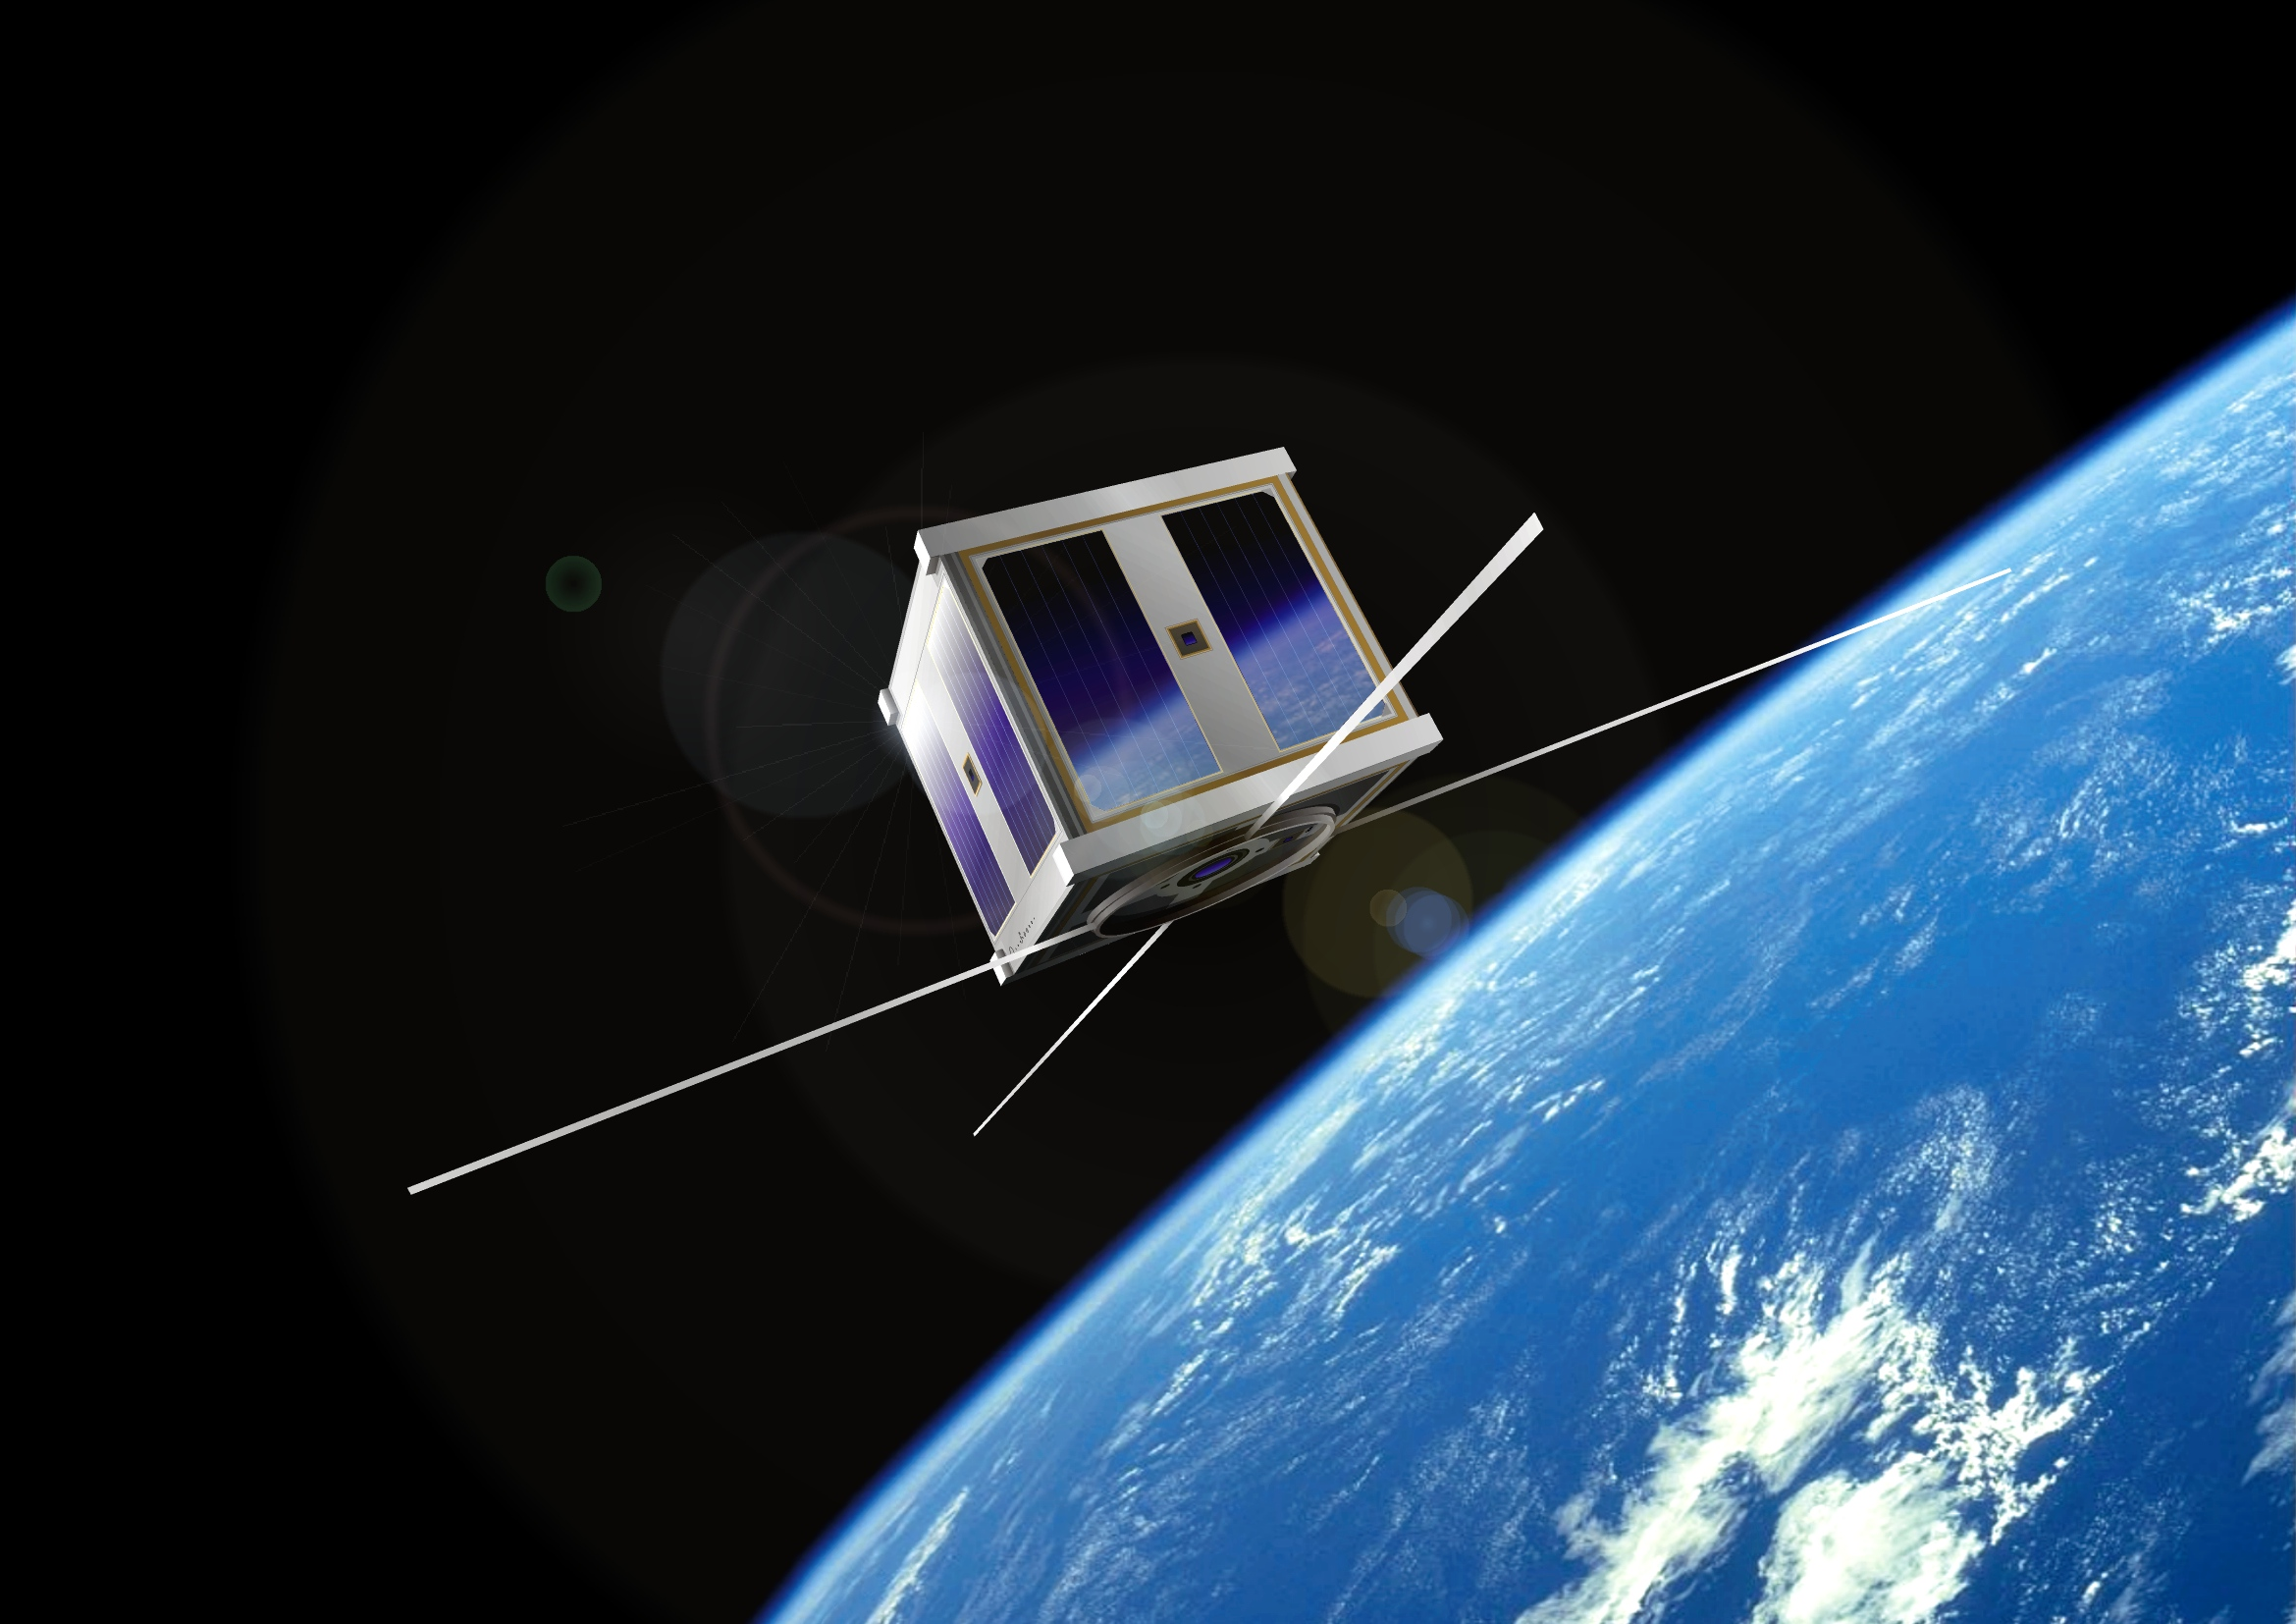
\includegraphics[width=0.8\textwidth]{figures/aau-sat}
\label{fig:forside}
\end{figure}
  \vspace{0.6 cm}
  \begin{center}
%    {\large
%      2. Semester Project Report %Insert document type (e.g., Project Report)
%    }\\
    \vspace{0.2cm}
    {\Large
      Group 17gr931%Insert your group name or real names here
    }
  \end{center}
  \begin{center}
  Aalborg University\\
  Control \& Automation\\
  Fredrik Bajers Vej 7\\
  DK-9220 Aalborg
  \end{center}
\end{titlepage}

\clearpage	%frontpage doh
\cleardoublepage
%\begin{document} 
%\thispagestyle{empty}
%\begin{titlepage}
\begin{nopagebreak}
{\samepage 

\begin{tabular}{r}
\parbox{\textwidth}{  \raisebox{-15mm}{
\includegraphics[height=3cm]{figures/aaulogo-en.png}}
\hfill \hspace{2cm} \parbox{8cm}{\begin{tabular}{l} %4.90
{\small \textbf{\textcolor{aaublue}{\colorbox{white}{9\textsuperscript{th} Semester, Project}}}}\\
{\small \textbf{\textcolor{aaublue}{School of Information and}}}\\
{\small \textbf{\textcolor{aaublue}{Communication Technologies}}}\\ 
{\small \textbf{\textcolor{aaublue}{Control and Automation}}}\\
{\small \textcolor{aaublue}{Fredrik Bajers Vej 7C}} \\
{\small \textcolor{aaublue}{9220 Aalborg}} \\
{\small \textcolor{aaublue}{\emph{en.aau.dk/education/master/control-automation}}}
\end{tabular}}}
\end{tabular}

\begin{tabular}{cc}
\parbox{7cm}{

\textbf{Title:}

Formation flying using pico-satellites\\ %\fxnote{Input project title}\\

\textbf{Theme:}

\small{
 Complex systems\\
}


\parbox{8cm}{


\textbf{Project Period:}\\
P9, Fall 2017\\
01/02/2017 - 20/10/2017\\
   
\textbf{Project Group:}\\
834\\ %\fxnote{Input group number}
  
\textbf{Participants:}\\
-\\
- \\
- \\

\textbf{Supervisors:}\\
Jesper Abilgaard Larsen \\ %\fxnote{Input supervisor}
}\\

\textbf{Prints:} -\\
\textbf{Pages:} -\\
\textbf{Appendices:} - (- pages)\\
\textbf{Attached:} 1 zip file\\
\textbf{Concluded:} 20/10/2017\\

\vfill } &
\parbox{7cm}{
  \vspace{.15cm}
  \hfill
  \begin{tabular}{l}
  {\textbf{Synopsis}}\bigskip \\
  \fbox{
    \parbox{6.5cm}{\bigskip
     {\vfill{\small This report describes the design and simulation of a control system on a AAU-CubeSat, which is a pico- satellite used for Low Earth Orbit flight.

The objective is to use a flight formation for monitoring Greenland, by having eight satellites equally distributed in orbit.

Two controllers must be designed, one to control the angle between the satellites using the drag force, and one for attitude control.  The drag force applied on the satellite depends on the cross section area which can be controlled using the orientation of the satellite.

A linear and a non-linear control method have been designed in order to compare the diferences between them.  
     \bigskip}}
     }}
   \end{tabular}}
\end{tabular}} %\vspace{1cm}

\textit{\phantom{A}Publication of this report's contents (including citation) without permission\\ \phantom{A}from the authors is prohibited}\\

\end{nopagebreak}
%\end{titlepage}
%\end{document}
\cleardoublepage
\chapter*{Preface}
This report has been written by group 931 on third semester in Control and Automation on Aalborg University.
References made before a full stop regards the sentence and reference after full stop regards the paragraph. Quotes are inside quotations marks and in cursive.
Attached to report is a zip file with:
\begin{itemize}
	\item -
	\item -
	\item -
	\item -
\end{itemize}
\vspace{2cm}

\textbf{Report by:}\\
\vspace{-5pt}
\begin{table}[H]
	\centering
	\begin{tabular}{c c c}
		\underline{\phantom{JAERJAERJAERJAERGO}} & \phantom{cookies} & \underline{\phantom{JAERJAERJAERJAERGO}} \\
		-		& \phantom{cookies} &  -		\\
		&&\\
		\multicolumn{3}{c}{\underline{\phantom{JAERJAERJAERJAERGO}}}\\
		\multicolumn{3}{c}{- }\\				
						
	\end{tabular}
\end{table}


\pagebreak


\tableofcontents         %     weather or not you want to create it.
\cleardoublepage

\pagenumbering{arabic} %use arabic page numbering in the mainmatter
\fancyfoot[RO,LE]{\thepage \text{ of} \pageref{LastPage}}
\fancyfoot[RE,LO]{17gr834}
\fancyhead[RE,LO]{}
\fancyhead[RE,LO]{\color{aaublue}\small\nouppercase\leftmark} %even page - chapter title
\pagestyle{fancy}

%||||||||||||||||||||||||||||||||||||||||||||||||||||||||||||||||
%|||||||       Set Section and chapters as input below   ||||||||
%||||||||||||||||||||||||||||||||||||||||||||||||||||||||||||||||

\chapter{Introduction}\label{chap:Introduction}

\section{Problem statement}
%Design and implement a controller for attitude and position of several pico-satellites in orbit.
Design and implement a controller for controlling the individual distance between satellites using the drag force.
\section{Use-case}\label{sec:useCase}
In this project, the concept of a formation flight of satellites will be used for the purpose of monitoring. Denmark has a small island called Greenland, where the Danish Government needs to monitor it. One method is to have a formation of satellites going around the orbit and when they are located in the northern hemisphere, the satellites will point down and look towards Greenland. 

One of the essentials in formation flight is choosing the number of satellites in orbit. Therefore, in order to have a continuous coverage, a distributed satellite system composed of six satellites equally distributed are chosen, compared with two or four satellites where communication between each other will be poor.
% After the surveillance, the concept is to change the attitude and having a control of the distance between them as they are in orbit.

The task the satellite has to perform is acquiring data by flying around Greenland, using radio signals and taking pictures.
%This gives two main objectives for the satellite: 
%\vspace{-0.5cm}
%\begin{itemize}
%	\item In formation flight one of the main challenges is to find and detect the position 
%	\item Acquiring data by flying around Greenland, using radio signals and taking pictures
%	\item Studying the orbital dynamic model by looking at one satellite neighbours 
%	\item Attitude and orbit determination using momentum wheels.
%\end{itemize}


\chapter{System Description}\label{chap:systemDescribtion}
The overall idea of the project is to consider more than one satellites flying in formation., with a certain distance in between and with the purpose of maintaining that distance by exchanging information. As a proof of concept, an AAU-CubeSat will be used, by choosing six AAU-CubeSat that orbit the Earth like is shown in  \figref{fig:1}. Therefore, a control system is developed, where the six satellites are nodes and they represent periods. Each satellite can only communicat with his two neighbour. In this project, all CubeSat's will be assumed identical, where each satellite needs to fulfill a few requirements stated in \chapref{chap:requirements}. Moreover, a full-scale implementation of the system will not be possible, therefore, the whole system will be simulated using MATLAB and Simulink. 
%
\begin{figure}[H]
	\centering
	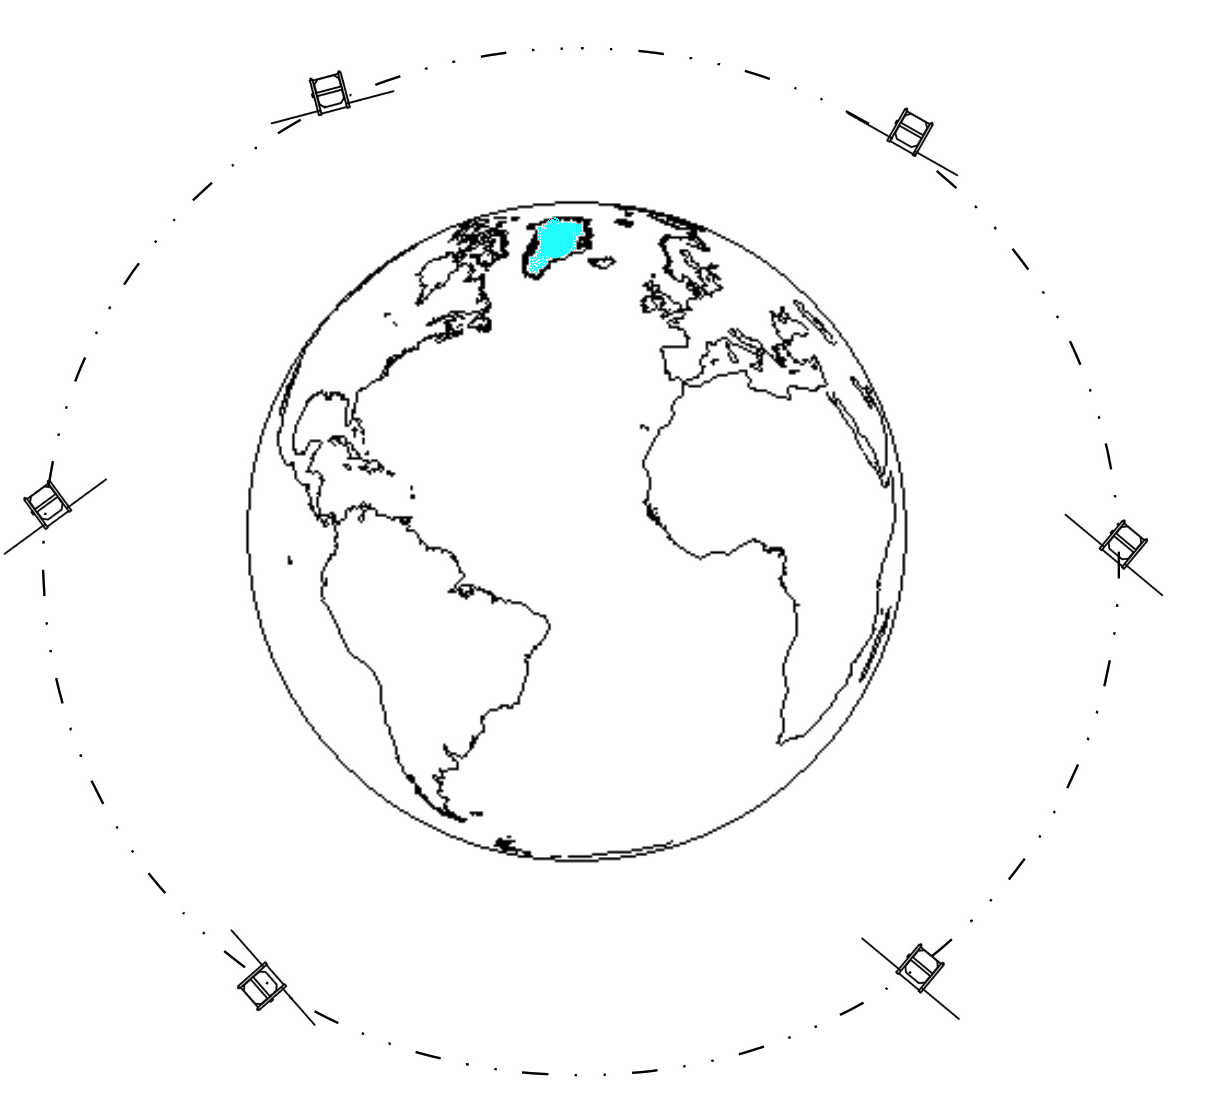
\includegraphics[width=0.6\linewidth]{figures/earth}
	\caption{desc.}
	\label{fig:1}
\end{figure}
%
\subsection{About AAU-CubeSat}
The AAU-CubeSat shown in \figref{fig:pico} is a pico-satellite developed by Stanford University, but assembled at Aalborg University by students and used mainly for Low Earth Orbit (LEO)  tests.
\begin{figure}[H]
	\centering
	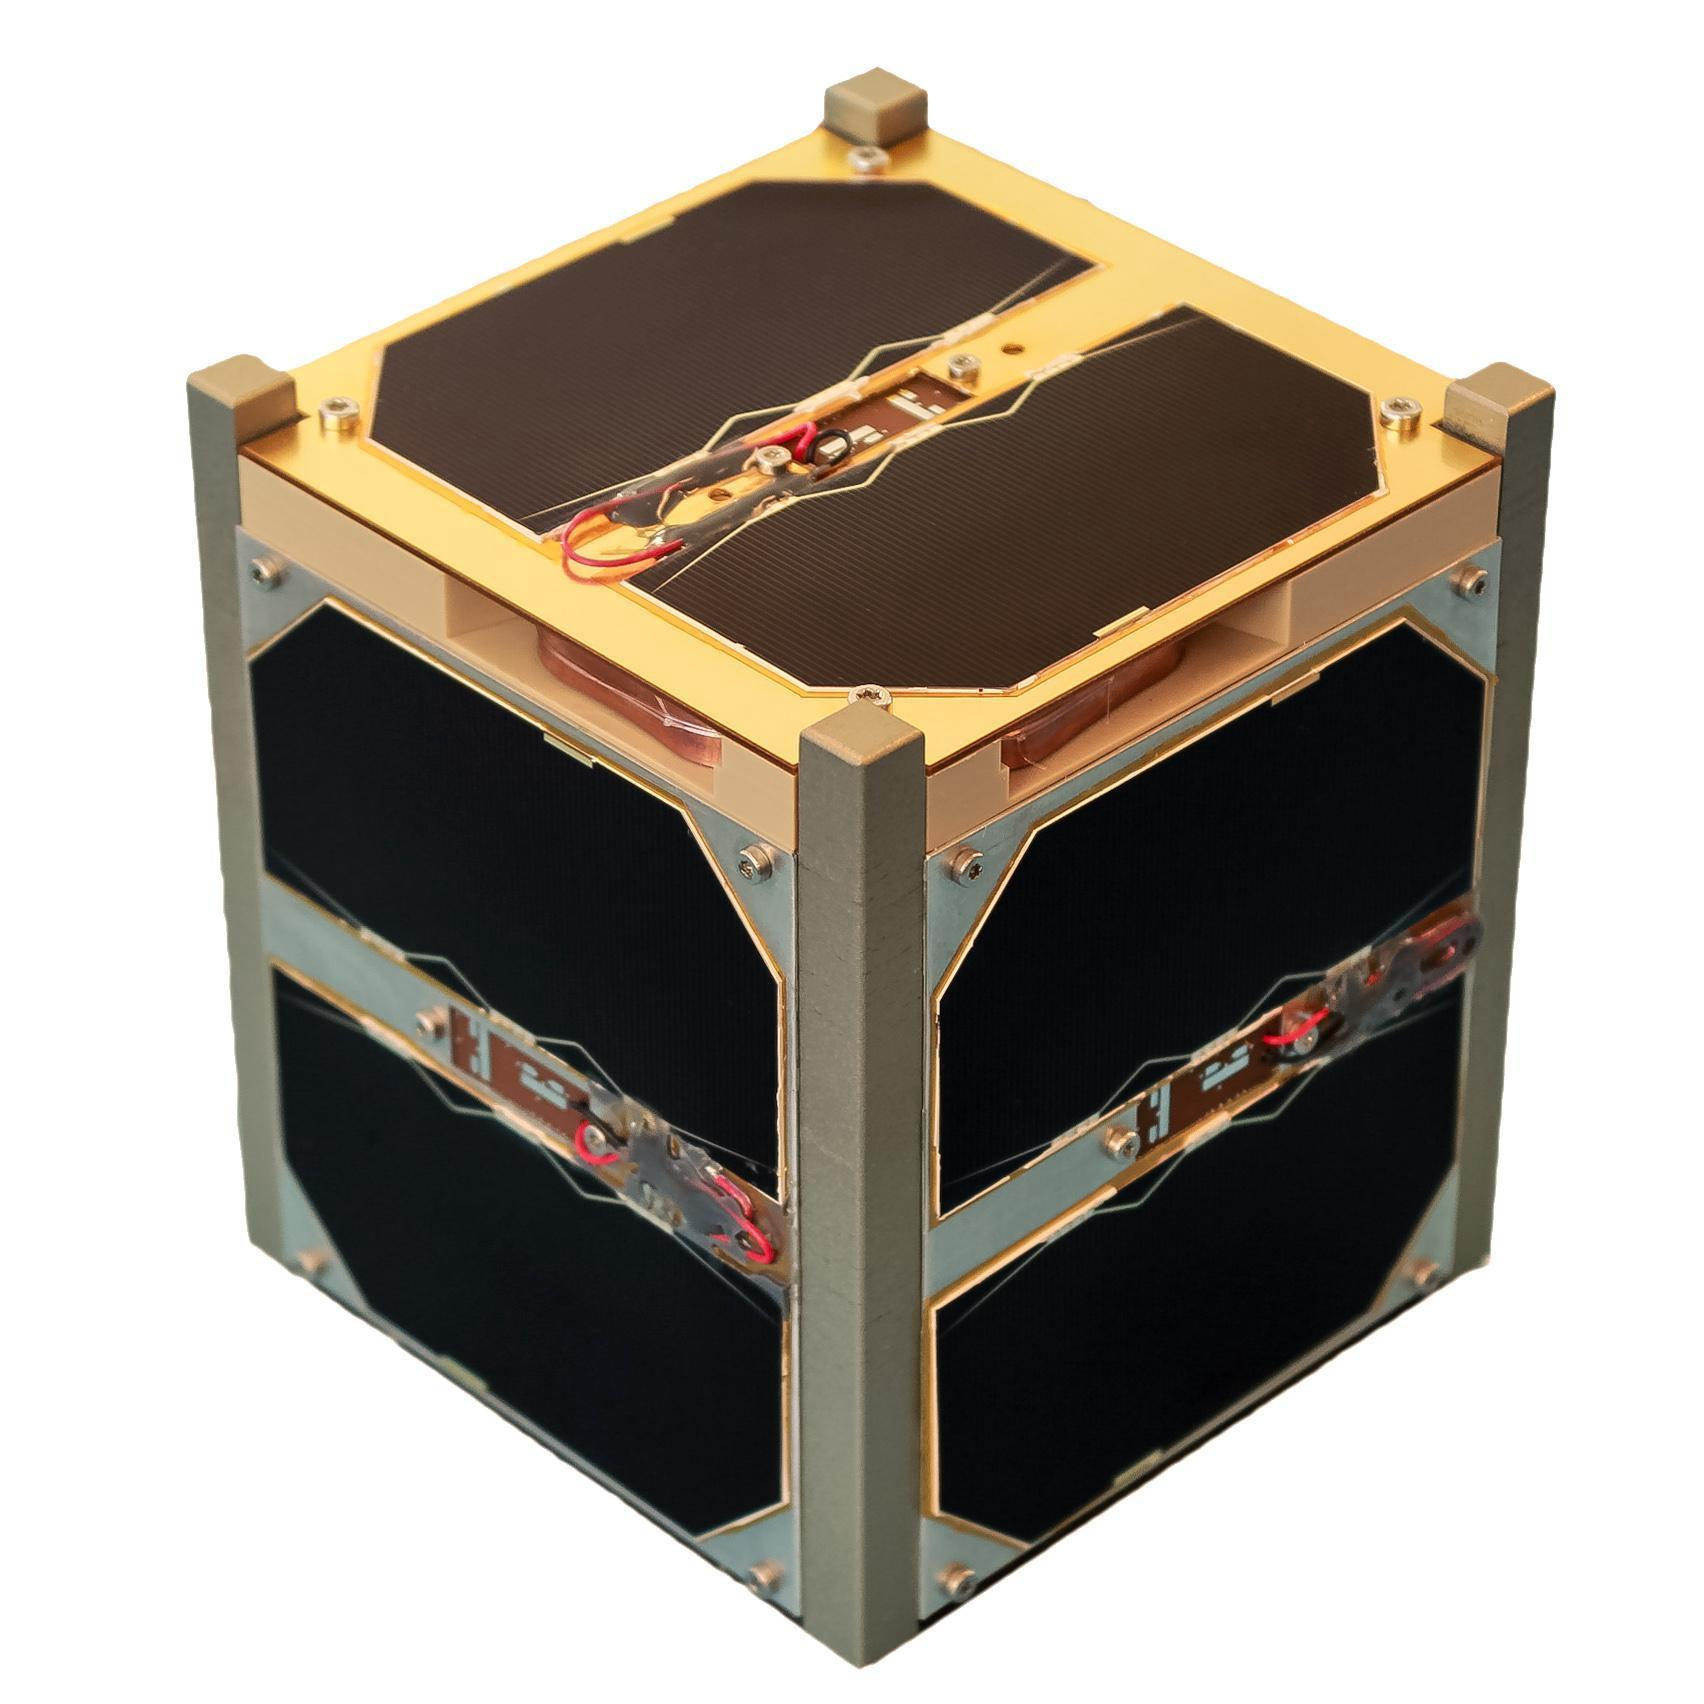
\includegraphics[width=0.3\linewidth]{figures/aau_cubsat}
	\caption{descrip}
	\label{fig:pico}
\end{figure}
The pico-satellite is designed for LEO, therefore a few constraints are imposed. The CubeSat is limited in size and weight. The dimensions of the satellite are $10cm\times10cm\times10cm$, while the weight around 1 kg. \fxnote{ref}

In order place the CubeSat on the orbit, a deployment system is used, called P-POD \fxnote{ref} This system uses the force of a spring to launch the satellite into space. The satellite will be placed inside the launch rocket as payload. By using this system, an important advantage is reducing the cost of the launch.
%
\subsection{AAU-CubeSat actuators}
The selection of attitude control components is important in order to meet the performance requirements. For this project, three magnetorquers and three momentum wheels have been chosen as actuators. Initially, using only three momentum wheels has been considered, but the downside of using only momentum wheels is that some amount of momentum can be stored in the wheel, which will imply having a way to take back all that momentum and use it. Therefore, there are two ways to release that torque, one is to use magnetorquers and the second to use thrusters. \fxnote{ref}

\textbf{Magnetorquers} are wire coils which generate an electromagnetic field. The field interacts with the Earth magnetic field and a torque is generated for stabilizing the satellite. An important aspect of the magnetorquer is when the momentum wheel reaches a maximum speed and can no longer produce the torque (this is referred as wheel saturation'), so a magnetorquer is used to extract the momentum from the wheel.
%
\begin{table}[H]
	\begin{minipage}[b]{0.49\linewidth}
		\centering
		\begin{figure}[H]
			\centering
			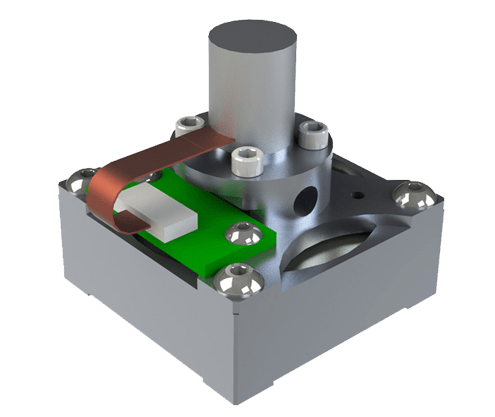
\includegraphics[width=0.5\linewidth]{figures/MW}
			\caption{Example of a reaction wheel for CubeSats}
			\label{fig:MW}
		\end{figure}
	\end{minipage}\hfill
	\begin{minipage}[b]{0.49\linewidth}
		\centering
		\begin{figure}[H]
			\centering
			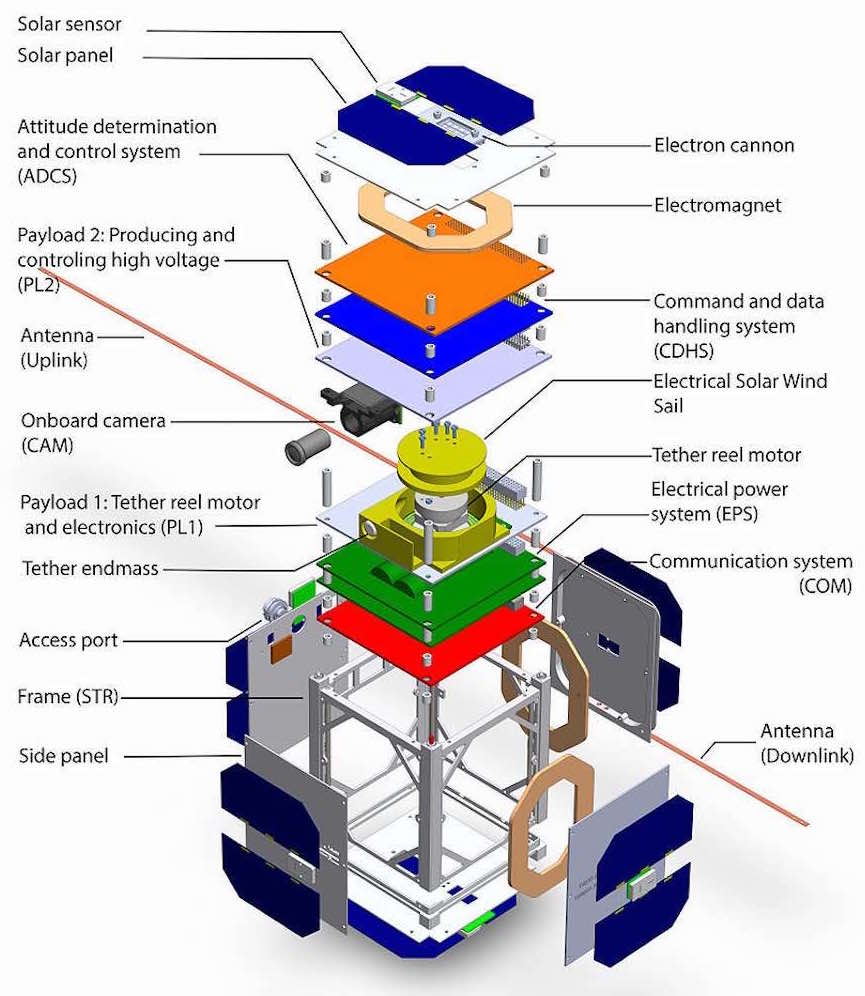
\includegraphics[width=1\linewidth]{figures/cubsat}
			\caption{Cubesat 3D view}
			\label{fig:cub}
		\end{figure}
	\end{minipage}
\end{table}
%
\textbf{Momentum wheels} shown in \figref{fig:MW} strength is that no information is needed about the magnetic field in order to control the CubeSat torque. These wheels are capable to store the momentum needed for maneuvering or pointing.
%
\subsection{AAU-CubeSat sensors}
The CubeSat can sustain itself using solar pannels [ref in fig 2.4] with in the middle a sun sensor, which provide a vector equal to the direction of the sun and also a magnetometer that gives a vector of the Earth's magnetic field. Whether the Earth’s magnetic field is measured, or the sun vector, the objective is to use these sensors to deliver vector solutions for determining the satellite’s pointing and rotation rates.

\textbf{Magnetometer} is a sensor used for attitude control, which measure the direction and intensity of the magnetic field. The atittude is determined from the magnetometer by comparing the measure magnetic field with a referance field.

\textbf{Sun sensor} is used for delivering a vector of measurements from the Sun. (ref to the fig 2.4 )
%
\subsection{Pointing accuracy}
The required pointing accuracy when acquiring a photo is based on the a height from the picture is taken, in this case around 700 km above the Earth surface is going to cover approximately ?? km. 




\chapter{Requirements}\label{chap:requirements}
Based on the use-case introduced and the available system a set of requirements are formulated.
%
\subsection*{System requirements}
%
\begin{enumerate}
	\item \textbf{The constellation shall be able to maintain a given distance} 
	\begin{itemize}
		\item []Measure the position of the satellites and using the drag force to control the velocity 
	\end{itemize}
	\item \textbf{The satellite should be able to turn twords target}
	\begin{itemize}
		\item[] Measure the current attitude of the satellites and to control it in order to achieve the specify orientation
	\end{itemize}
	
\end{enumerate}


\chapter{Modelling}
This chapter provides a description of the dynamic and kinematic equations of motion which constitute the basis for further analysis and description of the forces and/or disturbances, which may affect a rigid body within  Low Earth Orbit(LEO). The coordinate systems are defined first and then the model is derived the model for the satellite is defined based on rigid body dynamics and kinematics. 

In order to control the distance between two or more satellites in orbit, a mathematical description of the governing equations should be derived. Since precious work have been made in previous projects, and all the measurements are available, in-depth analysis it is deemed not necessary. 

\section{Coordinate systems}
\subsubsection{Earth Centered Inertial frame(ECI)}
\begin{figure}[H]
	\centering
	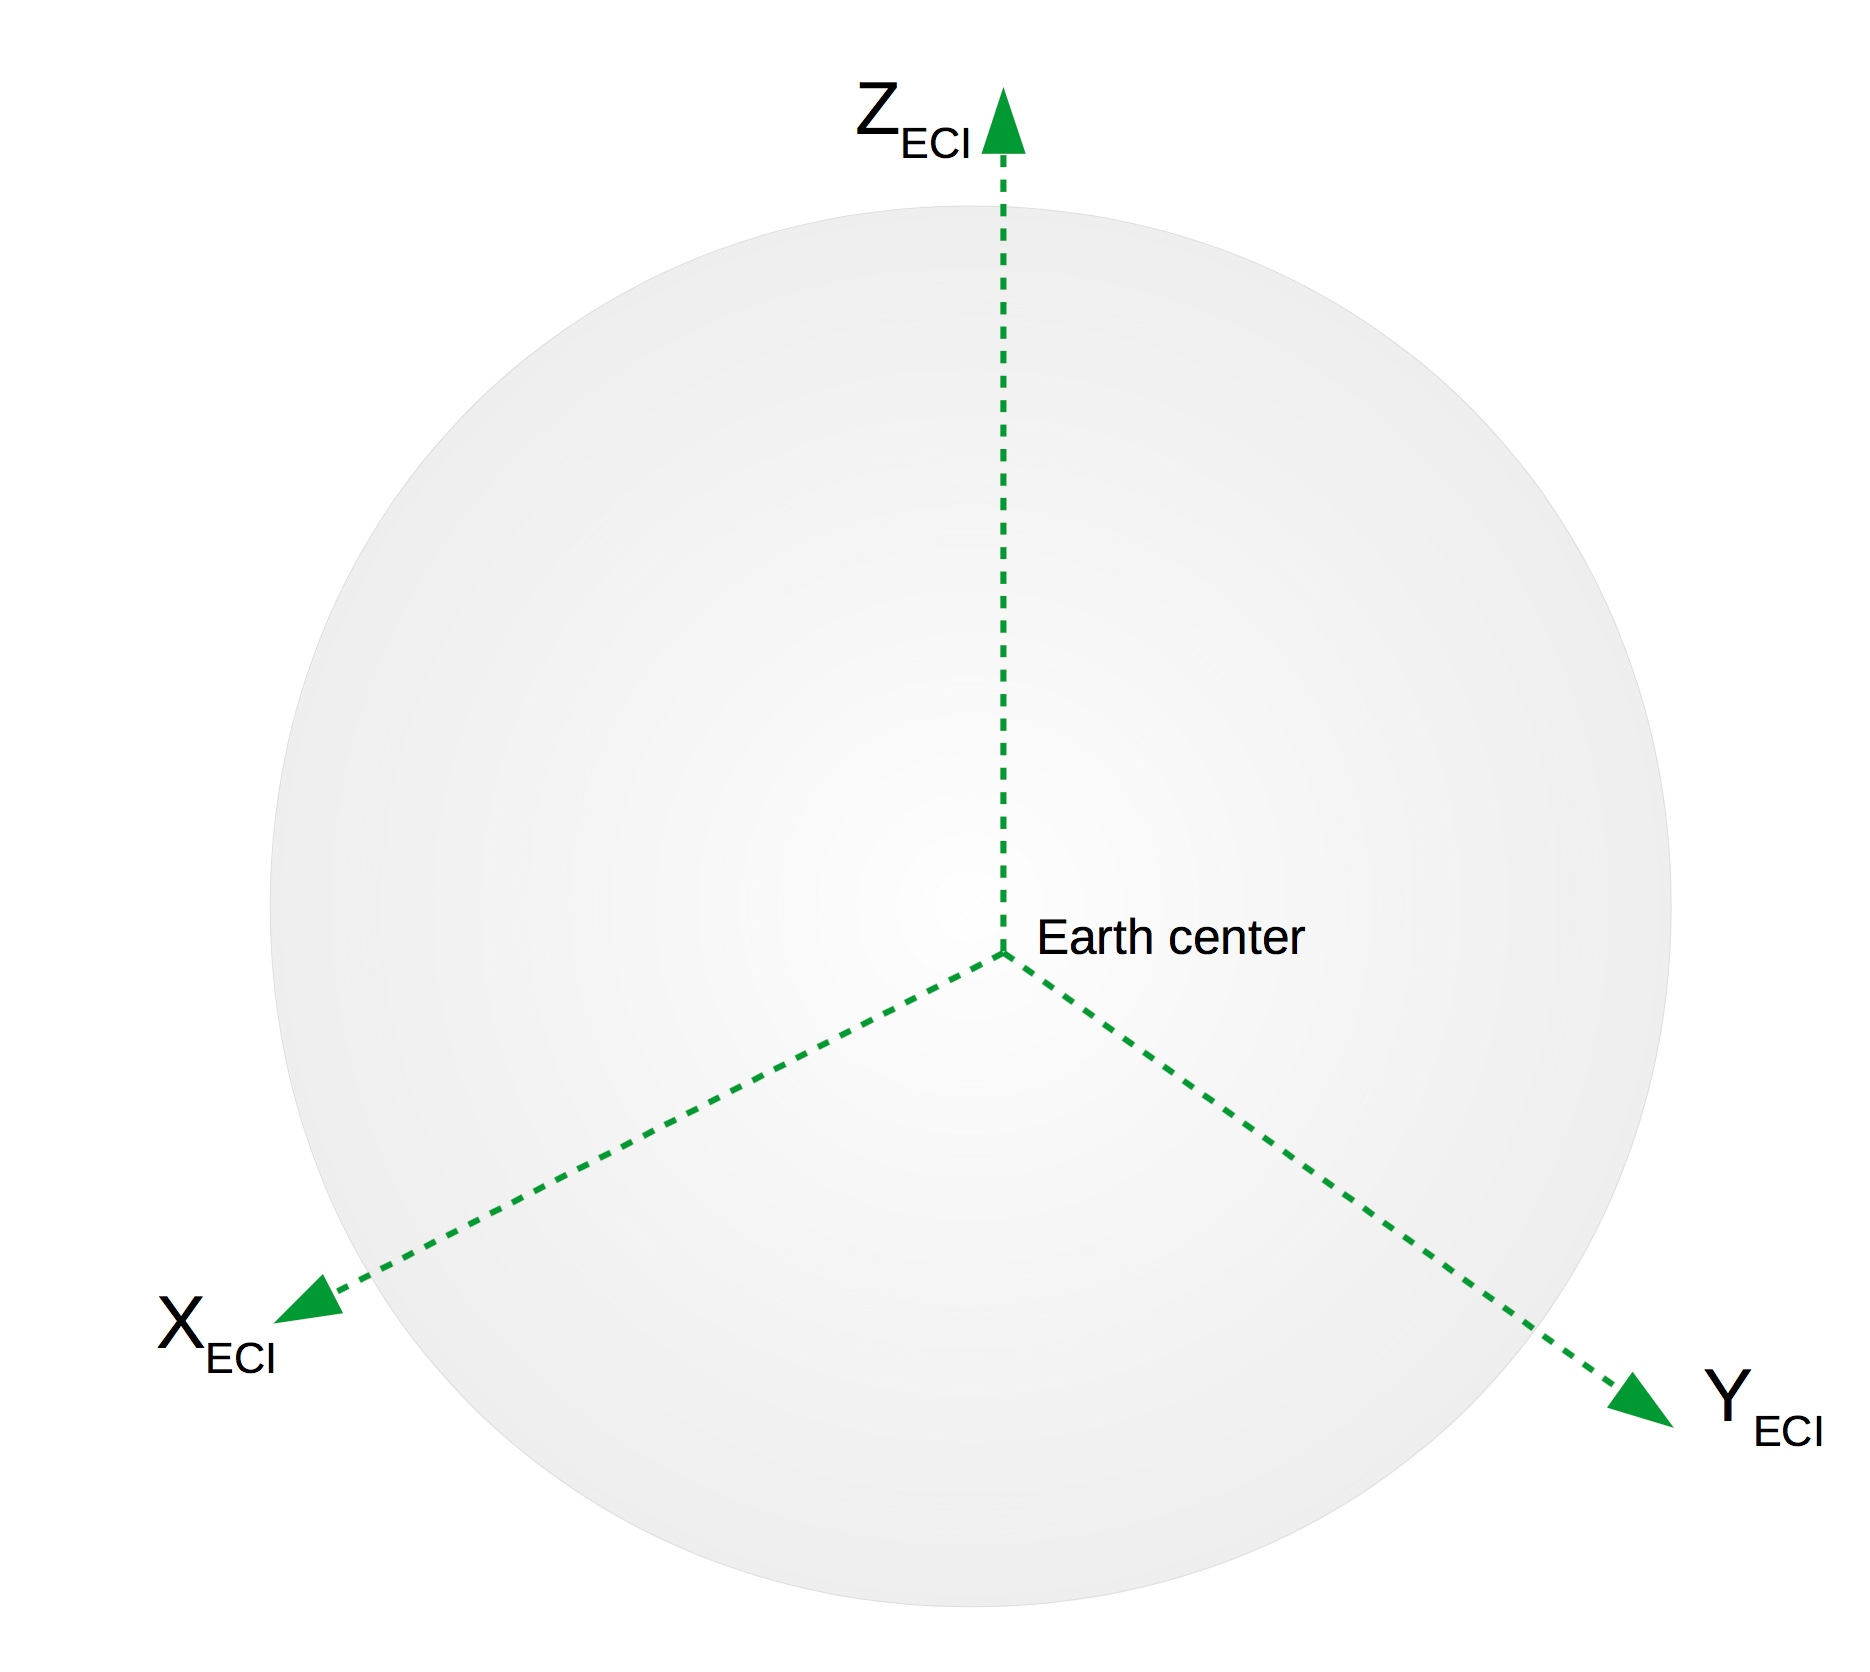
\includegraphics[width=0.5\linewidth]{figures/ECI}
	\caption{ECI coordinate frame}
	\label{fig:pico}
\end{figure}
In order to describe the orbit formation of the satellite, the ECI frame is used, since it can be seen as a non-accelerating frame. The $z$ axis is pointing through the geographical north pole, the $x$ axis is crossing from the point where the equatorial of the earth and the vernal equinox met and the $y$ axis is the cross product of $x$ and $z$ creating a right-handed coordinate system. 
%
\subsubsection{Orbit Reference frame(ORF)}
%
The orbit reference frame in Cartesian coordinates can be seen as a non-changing frame with respect the earth and the satellite. The $z$ axis always pointing at the nadir point and it is parallel to the $z_{e}$ axis o the inertial frame of the earth. The $x_{o}$ axis, it is parallel to the orbit plane and $y_{o}$ is the cross product of the $x_{o}$ and $z_{o}$. 
%
\subsubsection{Satellite Controller frame(SCF)}
%
In order to derive the kinematic equations, a controller reference frame should be specified. It is located in the center of mass of the satellite and it is defined such that the axis of higher inertia $z_{c}$ pointing in the center of ECI and the $x_{c}$ axis with the smallest inertia, pointing along with  the orbit's $x_{o}$ 
\section{Kinematics}
This section will provide the orbit-attitude determination of the satellite using quaternion representation. Since the differential drag control method is based on the rotation of the satellite in order to achieve the effective cross-sectional area, a notation with respect the collaborating frames should be obtained.     
%
\section{Dynamic Model}
In order to describe the behavior of the satellite a dynamic model based on reaction wheels and by using Euler's equation of motion has been derived.   
%
Euler's equation of motion describing the rotation of a rigid body is given by: \fxnote {ref}
% 
\begin{flalign}
	\dot{L} = {N_{tot}- \omega }{\times {L}}
	\label{eq:eulerequation}
\end{flalign}
% 
where $N_{tot}$ represents all the external torques caused from the actuator and the disturbances, $\omega$ is the angular velocity of the satellite and $L$ is the total angular momentum of the satellite and the reaction wheels, given by:
%
\begin{flalign}
	{L} = {I_{s}}{\omega}+{h_{tot}}
	\label{eq:angularmomentum}
\end{flalign}
%
where $h_{tot}$ is the vector of the angular momentum of the wheels $[h_{1} h_{2} h_{3}]^{T}$, all seen in the satellites coordinate system and $I_{s}$ is the inertia matrix of the satellite.
%
Inserting the equation \eqref{eq:angularmomentum} into \eqref{eq:eulerequation} we obtain
%
\begin{flalign}
	{\frac{d}{dt}(I_{s}{\omega})+\dot{h}_{(tot)}} ={N_{tot}-\omega}     {\times  ({I_{s}}{\omega} +{h_{tot}})}
	\label{eq:angularmomentum2}
\end{flalign}
For three reaction wheels attached at the body coordinate system which are the axis roll, pitch and yaw, three equations shall be derived. The derivation of the three equations of motion along with the diagonal inertia matrix can be found in the \label{Appendix A}.      
%
For the ease of notation, the cross product can be written as matrix operation using the $S()$ representing the skew symmetric matrix. Solving for $\dot{\omega}$ the dynamic equation can be written as 
%
\begin{flalign}
	{\dot{\omega}}={-I_{s}^{-1}S(\omega)I_{s}^{-1}\omega-I_{s}^{-1}S(\omega)h_{tot}-I_{s}^{-1}\dot{h}_{(tot)}+I_{s}^{-1}N_{tot}}
	\label{eq:angularmomentum3}
\end{flalign} 
%
The rate of change in angular momentum $\dot{h_{tot}}$ can be absorbed from the controller. This can be written as:
%
\begin{flalign}
	{\dot{h}_{(tot)}} ={-N{c}}
	\label{eq:rate of change}
\end{flalign}
%
where the negative sign denotes the absorbed momentum. The total torque from external disturbances can be written as $N_{dis}$. Rearranging, equation \eqref{eq:angularmomentum3} now reads 
%
\begin{flalign}
	{\dot{\omega}(t)} ={-I_{s}^{-1}S(\omega)I_{s}\omega(t)-I_{s}^{-1}S(\omega)h_{tot}+I_{s}^{-1}N_{c}(t)+I_{s}^{-1}N_{dis}(t)}
	\label{eq:angularmomentum4}
\end{flalign}
%
which constitute the dynamics of the satellite with three reaction wheels. At the final equation \eqref{eq:angularmomentum4} is shown the time dependency of the variables. 
%
\section{Disturbance Models}\label{sec:useCase} 
\subsection{Gravitational torque}
An unbalanced satellite in orbit is subjected to a torque due to the gravitational torque. Assumed that the earth is a point mass and the satellite is a rigid body, the gravitational torque can be estimated. Each infinitesimal element of the satellite of mass \textit{$dm_i$} is subjected to an infinitesimal force \textit{$dF_i$} that can be calculated thanks to Newton's law of universal gravitation.
\[
dF_i = -G\frac{m_{earth}}{R_i^2}dm_i \cdot \hat{R_i}
\]
where \textit{G} is the gravitational constant, \textit{$m_{earth}$} is the mass of the earth and \textit{$R_i^2$} is the vector from the earth to the infinitesimal element of the satellite. \\
The moment of the gravitational force about the geometric center is calculated as the formula:
\[
N_{gra} = \int_{sat} r_i \times dF_i 
\]
with $r_i$ is the vector from the geometric center to the infinitesimal element. $r_i$ can be written as the sum of the vector from the geometric vector to the mass center $r_{g,m}$ and the vector from the mass center of the element $r_{m,i}$. Therefore, the expression of the gravitational torque is simplified:
\begin{align*}
	N_{gra} &= \int_{sat} r_{g,m} \times dF_i + \int_{sat} r_{m,i} \times dF_i \\
	&= \int_{sat} r_{g,m} \times -G\frac{m_{earth}}{R_i^2}dm_i \cdot \hat{R_i} + \int_{sat} r_{m,i} \times -G\frac{m_{earth}}{R_i^2}dm_i \cdot \hat{R_i}
\end{align*}
We can assumed that $r_{m,g} << R_i$ and $R_i$ can be supposed constant and equals to the vector from the center of the earth to the geometric center of the satellite $R_{e,g}$. Thus, The second term is null by definition of the mass center.
\[
\Rightarrow N_{gra} = G\frac{m_{sat} \cdot m_{earth}}{R_{e,g}^2} \cdot (\hat{R_i} \times r_{g,m})
\]
The position of the center of mass was measured for the previous project and is eqals to [?;?;?] in the frame of the satellite. Therefore, $r_{g,m,i}$ can be expressed in the inertial frame as following:
\[
[r_{g,m,i};0] = q_{i,s} \otimes [?;?;?.0] \otimes q_{i,s}*
\]
where $q_{i,s}$ is the quaternion that represents the rotation of the satellite in the inertia frame and $\otimes$ is the quaternion multiplication. Thus, the moment of force can be calculated by this expression above.
  7890
\chapter{Acceptance test} \label{chap:acceptanceTest}
The system is tested to see if it fulfills the requirements put up (\chapref{chap:requirements}).

\subsection{The formation shall be able to maintain a given angle within 45$^{\circ}$.}
%
The requirement was to test if the system of satellites can create and maintain a certain distance between them which is measured with an angle of 45$^{\circ}$ from the center of the earth using the drag force. A linear quadratic controller has been designed. It is assumed that the satellites can turn instantly to the direction of the desired drag force. So the output of the controller can be seen as the applied drag force to the satellite.        
%
The satellites are assumed to start from the same place. Two cases have been tested, a global algorithm where the formation converge to $u_{min}$ and distributed algorithm where the formation converge to $u_medium$. In both cases the controller reacts well even if the convergence in the global algorithm is faster.
%
In conclusion the requirement is fulfilled in both cases since the system is able to create an maintain a constant angle.  
\subsection{Each satellite shall be able to change its orientation.}
%



\chapter{Conclusion}
The overall objective of this project was to consider several satellites flying in formation with the purpose of pointing towards a target. In order to reach this goal, two controllers were designed: one for controlling the angle between satellites using the drag force and another one for attitude control in order to be able to rotate the satellite to the desired orientation.

First, for designing a controller for the angle, the relative dynamics between two satellites are analyzed. Therefore, an LQR controller is implemented to control the angle between two satellites. The simulations showed that the LQR performed properly. Additionally, two algorithms for formation control are designed, a global and distributed algorithm. Both algorithms are working as intended, where the angles between neighbour satellites converged to the desired angle of 45$^{\circ}$, with the mention that in the distributed algorithm case the convergence rate will be slower compared with the global algorithm.

Afterwards, two control methods to obtain the desired orientation of the satellite has been implemented. The first method is a state feedback which is a linear control method. For implementing this controller the equation of motion need to be linearized. The second method is using a non-linear control method called sliding mode control. The results from sliding mode control showed that the error quaternion converged better compared to state feedback control, but in this case, the state feedback is deemed to be more suitable. Besides, the sliding mode convergence is better, but due to the fact that the control law is more complex, the satellite controler will need more computation time. 

In conclusion, some acceptance tests have been made to establish that the requirements accomplished. 

%%% Bibliography %%%
%\printbibliography
%\cleardoublepage
%---------- Appendix Below ----------------------------------------
\appendix

\chapter{Appendix A }\label{sec:motorappendix}
%
\section{Derivation of Equation of motion}
The general Euler's rotation equation with three reaction wheels aligned on the satellite body axis are derived as
%
\begin{flalign}
	{I_{1} \dot{\omega_{1}}} ={(I_{2}-I_{3})\omega_{2}\omega_{3}+N_{1}-\omega_{2}h_{3}+\omega_{3}h_{2}}
	\label{eq:angularmomentum2Appedix1}
\end{flalign}
%
\begin{flalign}
	{I_{2} \dot{\omega_{2}}} ={(I_{3}-I_{1})\omega_{1}\omega_{3}+N_{2}-\omega_{3}h_{1}+\omega_{1}h_{3}}
	\label{eq:angularmomentum2Appedix2}
\end{flalign}  
%
\begin{flalign}
	{I_{3} \dot{\omega_{3}}} ={(I_{1}-I_{2})\omega_{1}\omega_{2}+N_{3}-\omega_{1}h_{2}+\omega_{2}h_{1}}
	\label{eq:angularmomentum2Appedix3}
\end{flalign}
%
The equation in compact form has been written as 
%
\begin{flalign}
	{\dot{\omega}} ={-I_{s}^{-1}S(\omega)I_{s}^{-1}\omega-I_{s}^{-1}S(\omega)h_{tot}-I_{s}^{-1}\dot{h}_{(tot)}+I_{s}^{-1}N_{tot}}
	\label{eq:angularmomentum2Appedix4}
\end{flalign}
%
where $S(\omega)$ is the skew symmetric matrix given by
%
\begin{flalign}
	{S{\omega}}
	= 
	\begin{bmatrix}
		0& -\omega_{3}& \omega_{2} \\
		\omega_{3}& 0&-\omega_{1}  \\ 
		-\omega_{2} & \omega_{1} &0
	\end{bmatrix} 
	\label{eq:skewsymmetricmatrix}
\end{flalign}
%
and the angular momentum of the reaction wheels as $h_{tot}=[h_1 \ h_2 \ h_3]^{T}$.
\subsection{Inertia matrix}
%
The inertia matrix for a solid cuboid of height $z$ , width $y$, and depth $x$, amd mass $m_{i}$ with respect the center of mass is given by 
%
\begin{flalign}
	{I}_{i}
	= 
	\begin{bmatrix}
		\frac{1}{12} m_i(z^{2}+y^{2}) &0&0 \\
		0&  \frac{1}{12}m_i(z^{2}+x^{2})&0   \\ 
		0 & 0 &\frac{1}{12} m_i(x^{2}+y^{2}
	\end{bmatrix} 
	\label{eq:inertiaTensorMatrix}
\end{flalign}
%
It is assumed that the Cube have a symmetric mass distribution around the axis of rotation to simplify the inertia matrix.  
With the mass distributed evenly and the axis of rotation being around one of the tree axis, the off diagonal term of the inertia matrix are equal to zero. These terms are also referred to as cross products of inertia.
\chapter{Derivation of relative dynamics equations} \label{chap:B}
The vector position from the centre of the Earth to the satellite 1 and the satellite 2 is given by
\begin{flalign}
\vec{p_1} &= R  \vec{\hat{x}} \\
\vec{p_2} &= R  \vec{\hat{x}} + x  \vec{\hat{x}} + y  \vec{\hat{y}}
\end{flalign}
the first time derivative and second time relative of $\vec{p_1}$ and $\vec{p_2}$ is computed:
\begin{flalign*}
\dot{\vec{p_1}} &= \dot{R}  \vec{\hat{x}} + R(\vec{w} \times \vec{\hat{x}}) 
\end{flalign*}
where $\vec{w}$ is the angular velocity vector and $\vec{w} = w  \vec{\hat{z}}$ due to the fact the position of the satellites stay all over the time in the plan $(\vec{\hat{x}},\vec{\hat{y}})$. Therefore, the first time derivative and the second time derivative are given by:
\begin{flalign*}
\dot{\vec{p_1}} &= \dot{R}  \vec{\hat{x}} + w R  \vec{\hat{y}} \\
\ddot{\vec{p_1}} &= \ddot{R}  \vec{\hat{x}} + w\dot{R}  \vec{\hat{y}} + \dot{w} R  \vec{\hat{y}} + w \dot{R}  \vec{\hat{y}} + wR  (\vec{w} \times \vec{\hat{y}}) \\
&= \ddot{R}  \vec{\hat{x}} + 2w\dot{R}  \vec{\hat{y}} - w^2R  \vec{\hat{x}} \\
\dot{\vec{p_2}} &= \dot{\vec{p_1}} +  \dot{x}  \vec{\hat{x}} + x w  \vec{\hat{y}} + \dot{y}  \vec{\hat{y}} - y w  \vec{\hat{x}} \\
&= \dot{\vec{p_1}} + (\dot{x} - yw)  \vec{\hat{x}} + (xw + \dot{y})  \vec{\hat{y}} \\
\ddot{\vec{p_2}} & = \ddot{\vec{p_1}} + (\ddot{x} - \dot{y}w - y\dot{w})  \vec{\hat{x}} + (\dot{x} - yw) w  \vec{\hat{y}} + (\dot{x}w + x\dot{w} + \ddot{y})  \vec{\hat{y}} - (xw + \dot{y}) w  \vec{\hat{x}} \\
&= \ddot{\vec{p_1}} + (\ddot{x} - 2\dot{y}w - y\dot{w} - xw^2)  \vec{\hat{x}} + (\ddot{y} + 2\dot{x}w + x\dot{w} - yw^2)  \vec{\hat{y}}
\end{flalign*}
Furthermore, The Newton law gives:
\begin{flalign}
	m\ddot{\vec{p_1}} &= \vec{F_{grav,1}} + \vec{F_{drag,1}} + \vec{F_{dist,1}}	\label{eq:l3} \\
	m\ddot{\vec{p_2}} &= \vec{F_{grav,2}} + \vec{F_{drag,2}} + \vec{F_{dist,2}} 	\label{eq:l4} \\
	\Rightarrow \ddot{\vec{p_2}} - \ddot{\vec{p_1}} &= \frac{1}{m}(\Delta \vec{F_{grav}} + \Delta \vec{F_{drag}} + \Delta \vec F_{dist}) 	\label{eq:l5}
\end{flalign}
with m is the mass of both satellites. The gravity is given by the universal law of gravitation:
\begin{flalign*}
\frac{\vec{F_{grav,1}}}{m} &= -G\frac{m_{earth}}{||\vec{R}||^3} \vec{R} \\
\frac{\vec{F_{grav,2}}}{m} &= -G\frac{m_{earth}}{||\vec{R} + \vec{r}||^3} (\vec{R} + \vec{r})
\end{flalign*}
where $\vec{r} = (x,y)$ is the vector from the satellite 1 to the satellite 2. The denominateur can be approximated using:
\begin{flalign*}
||\vec{R} + \vec{r}||^{-3} &= ||\vec{r}|| \\
%||\vec{R} + \vec{r}||^{-3} &= ||(\vec{R} + \vec{r})\cdot(\vec{R} + \vec{r})||^{\frac{-3}{2}} \\
%&= ||\vec{R} \cdot \vec{R} + \vec{r} \cdot \vec{r} + 2\vec{R} \cdot \vec{r}||^{\frac{-3}{2}} \\
%&= R^{-3}||1 + \frac{\vec{r} \cdot \vec{r}}{R^2} + 2\frac{\vec{r} \cdot \vec{R}}{R^2}||^{\frac{-3}{2}}
\end{flalign*}
%Due to the fact the $r << R$, the second term can be neglected and by using the approximation $(1 + x)^q = 1 + qx$ when $x << 1$. The expression can be approximated by:
%\begin{flalign*}
%||\vec{R} + \vec{r}||^{-3} &= R^{-3}(1 - 3\frac{\vec{r} \cdot \vec{R}}{R^2}) \\
%&= R^{-3}(1 - 3\frac{x}{R})
%\end{flalign*} 
and thus, the difference between the gravity force on satellite 2 and the the gravity force on 1 is:
\begin{flalign*}
\vec{F_{grav,2}} - \vec{F_{grav,1}} &\approx -\frac{\mu}{R^3}\vec{r} \\
%\vec{F_{grav,2}} - \vec{F_{grav,1}} &\approx -G \frac{m_{earth}}{R^3} ((1 - 3\frac{x}{R}) (\vec{R} + \vec{r}) - \vec{R}) \\
%&\approx -G \frac{m_{earth}}{R^3} (\vec{r} - 3x \cdot \vec{\hat{x}} + 3 \frac{x}{R} \vec{r}) \\
%&\approx -\frac{\mu}{R^3} (-2x \cdot \vec{\hat{x}} + y \cdot \vec{\hat{y}})
\end{flalign*} 
with $\mu = G  m_{earth}$, The drag force can be modelling be using \eqref{eq:teor}:
\begin{flalign*}
	\vec{F_{drag,1}} &= -u_1 ||\dot{\vec{p_1}}|| \dot{\vec{p_1}}\\
	& = -u_1 ||\dot{\vec{p_1}}|| (\dot{R}  \vec{\hat{x}} + wR  \vec{\hat{y}}) \\
	\vec{F_{drag,2}} &= -u_2 ||\dot{\vec{p_2}}|| \dot{\vec{p_2}} \\
	& = -u_2 ||\dot{\vec{p_2}}|| ((\dot{R} + \dot{x} - yw) \vec{\hat{x}} + (wR + xw + \dot{y})  \vec{\hat{y}})
\end{flalign*}
Therefore, the \eqref{eq:l3} becomes:
\begin{equation}
\left\{
	\begin{aligned}
		&\ddot{R} - w^2R = -\frac{\mu}{R^2} -\frac{u_1}{m} ||\dot{\vec{p_1}}|| \dot{R} + \frac{F_{dist,1,x}}{m} \\
		&2w\dot{R} + \dot{w}R = -\frac{u_1}{m} ||\dot{\vec{p_1}}|| wR + \frac{F_{dist,1,y}}{m}
	\end{aligned}
\right.
\end{equation}
and the \eqref{eq:l5} gives:
\begin{equation}
\left\{
	\begin{aligned}
		& \ddot{x} - 2\dot{y}w - y\dot{w} - xw^2 = -x\frac{\mu}{R^3} + \frac{u_1}{m} ||\dot{\vec{p_1}}|| \dot{R} - \frac{u_2}{m} ||\dot{\vec{p_2}}||(\dot{R} + \dot{x} - yw) + \frac{\Delta F_{dist,x}}{m}\\
		&\ddot{y} + 2\dot{x}w + x\dot{w} - yw^2 = -y\frac{\mu}{R^3} + \frac{u_1}{m}||\dot{\vec{p_1}}||wR - \frac{u_2}{m}||\dot{\vec{p_2}}||(wR + xw + \dot{y}) + \frac{\Delta F_{dist,y}}{m}
	\end{aligned}
\right.
\label{eq:l7}
\end{equation}
The operating point is the position ($x^{*},y^{*}$) of the satellite 2 in the frame of satellite. $x^{*}$ and $y^{*}$ can be computed from \figref{fig:operating_pt}.
\begin{figure}[H]
	\centering
	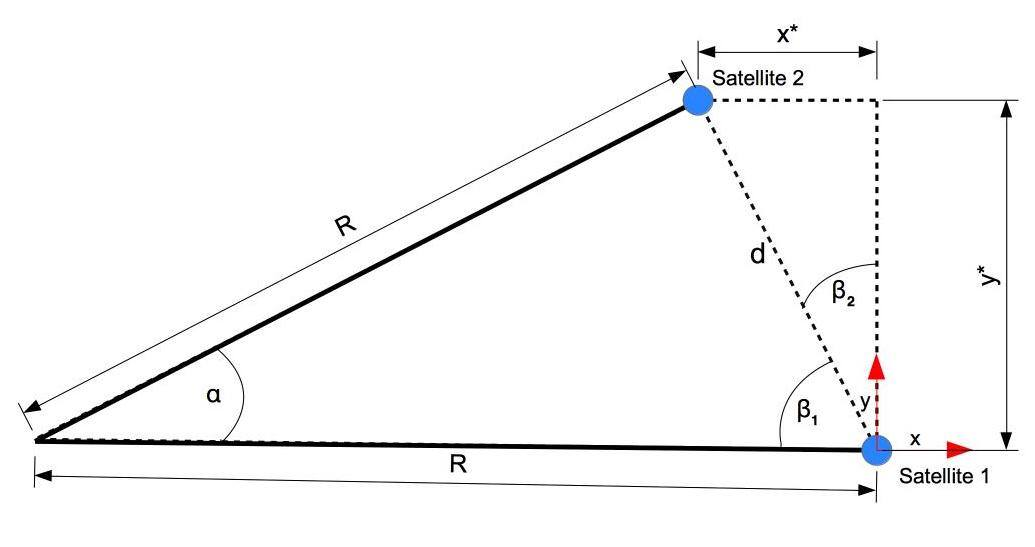
\includegraphics[width=0.75\linewidth]{figures/operating_point}
	\caption{Operating point}
	\label{fig:operating_pt}
\end{figure} 
Using trigonometry relations:
\begin{flalign*}
d &= 2Rsin(\frac{\alpha}{2}) \\
x^{*} &= -dsin(\beta_2) \\
&= -dsin(\frac{\alpha}{2}) \\
&= -2Rsin(\frac{\alpha}{2})^2 \\
y^{*}  &= dcos(\frac{\alpha}{2}) \\
&= 2Rsin(\frac{\alpha}{2})cos(\frac{\alpha}{2}) \\
&= Rsin(\alpha)
\end{flalign*}
with $\alpha$ is the desired angle between satellite and so $\beta_2 = 90^{\circ} - \beta_1 = 90^{\circ} - (90^{\circ} - \frac{\alpha}{2}) = \frac{\alpha}{2}$. Therefore we change the coordinate reference as following:
\begin{flalign*}
x &\Leftarrow x - x^{*}  \\
y &\Leftarrow y - y^{*}  
\end{flalign*}
Thus, the equations \eqref{eq:l7} become:
\begin{equation}
\left\{
\begin{aligned}
	& \ddot{x} - 2\dot{y}w - (y + y^{*})\dot{w} - (x + x^{*})w^2 = \\
	&-(x + x^{*})\frac{\mu}{R^3} + \frac{u_1}{m} ||\dot{\vec{p_1}}|| \dot{R} - \frac{u_2}{m} ||\dot{\vec{p_2}}||(\dot{R} + \dot{x} - (y + y^{*})w) + \frac{\Delta F_{dist,x}}{m}\\
	&\ddot{y} + 2\dot{x}w + (x + x^{*})\dot{w} - (y + y^{*})w^2 =\\
	& -(y + y^{*})\frac{\mu}{R^3} + \frac{u_1}{m}||\dot{\vec{p_1}}||wR - \frac{u_2}{m}||\dot{\vec{p_2}}||(wR + (x + x^{*})w + \dot{y}) + \frac{\Delta F_{dist,y}}{m}
\end{aligned}
\right.
	\label{eq:la1}
\end{equation}
%\subsection{Linearisation of the relative dynamics eqations} \label{sec:C}
%From the equations \eqref{eq:la1} and assuming that the radius is constant and the angular velocity equals to $w = \sqrt{\frac{\mu}{R^3}}$, a linearization of the system can be derived using some approximations. The state is defined as :
%\begin{flalign*}
%	s = [x \ \dot{x} \ y \ \dot{y}]^\mathsf{T}
%\end{flalign*}
%Moreover, the norm of the velocity of both satellite is assumed to be equal and to be constant ($||\vec{\dot{p_1}}|| = ||\vec{\dot{p_2}}|| = C$). Therefore, the nominal system is given by:
%\begin{equation}
%\left\{
%\begin{aligned}
%& \dot{s_1} = s_2 \\
%& \dot{s_2} = 2ws_4 - u_2\frac{y^{*}wC}{m} \\
%& \dot{s_3} = s_4 \\
%& \dot{s_4} = -2ws_2 - (u_2 - u_1)\frac{wRC}{m}
%\label{eq:statespaceassumption}  
%\end{aligned}
%\right.
%\end{equation}
%using the approximation $\dot{x}$, $y << y^{*}$ and $x, x^{*}$, $\frac{\dot{y}}{w} << R$. 
%

%%% Bibliography %%%
\printbibliography

%%% List of Corrections
\listoffixmes

\end{document}
